\documentclass[11pt,a4paper]{article}
\usepackage{TeX_definitions}
\geometry{left=2.4cm,right=2.4cm,top=2.4cm,bottom=2.4cm}
\graphicspath{{figures/}}
\hypersetup{colorlinks=true,linkcolor=blue,citecolor=blue,urlcolor=blue}

\title{Analysis 4-3: parameter identifiability of structural attenuation and factor strength}
\author{}
\date{\today}
\begin{document}
\maketitle

\section{Question}
Analysis 4-3 asks whether attenuation on the true graph can be distinguished from weaker pairwise couplings. The structural interpretation of $M_{\rho}$ is only defensible if $\rho$ is not simply absorbing changes in $\beta_{\mathrm{edge}}$.

\section{Method}
Standard graphical-model background and notation are treated in the usual way; see \cite{Koller2009}.


We evaluated a joint grid over $\rho$ and $\beta$, computed panel-level divergences, local identifiability scores, a diagnostic recovery panel, synthetic noiseless and noisy recovery, and best-case cross-family matches after $\beta$ optimisation.

\section{Results}
The diagnostic recovery panel retained eight high-value conditions: RG031 (high), RG100 (high), RG088 (high), RG087 (high), RG091 (high), RG111 (high), RG112 (high), RG114 (high). On this panel the noiseless exact-match rate is 1.0, so the parameters are identifiable in principle. Under noisy synthetic responses the exact-match rate falls to 0.3, with mean absolute errors 0.136587 for $\rho$ and 0.584921 for $\beta$. This is strong enough to justify joint modelling, but weak enough to show that the tradeoff is real.

The family robustness analysis is especially revealing. Once $\beta$ is optimised, attenuation collapses perfectly onto exact inference at the exact endpoint, but the best attenuation-versus-star match still leaves mean JS 0.027041. Structure rewrites therefore remain more robust than subtle within-graph attenuation contrasts.

\begin{figure}[H]
\centering
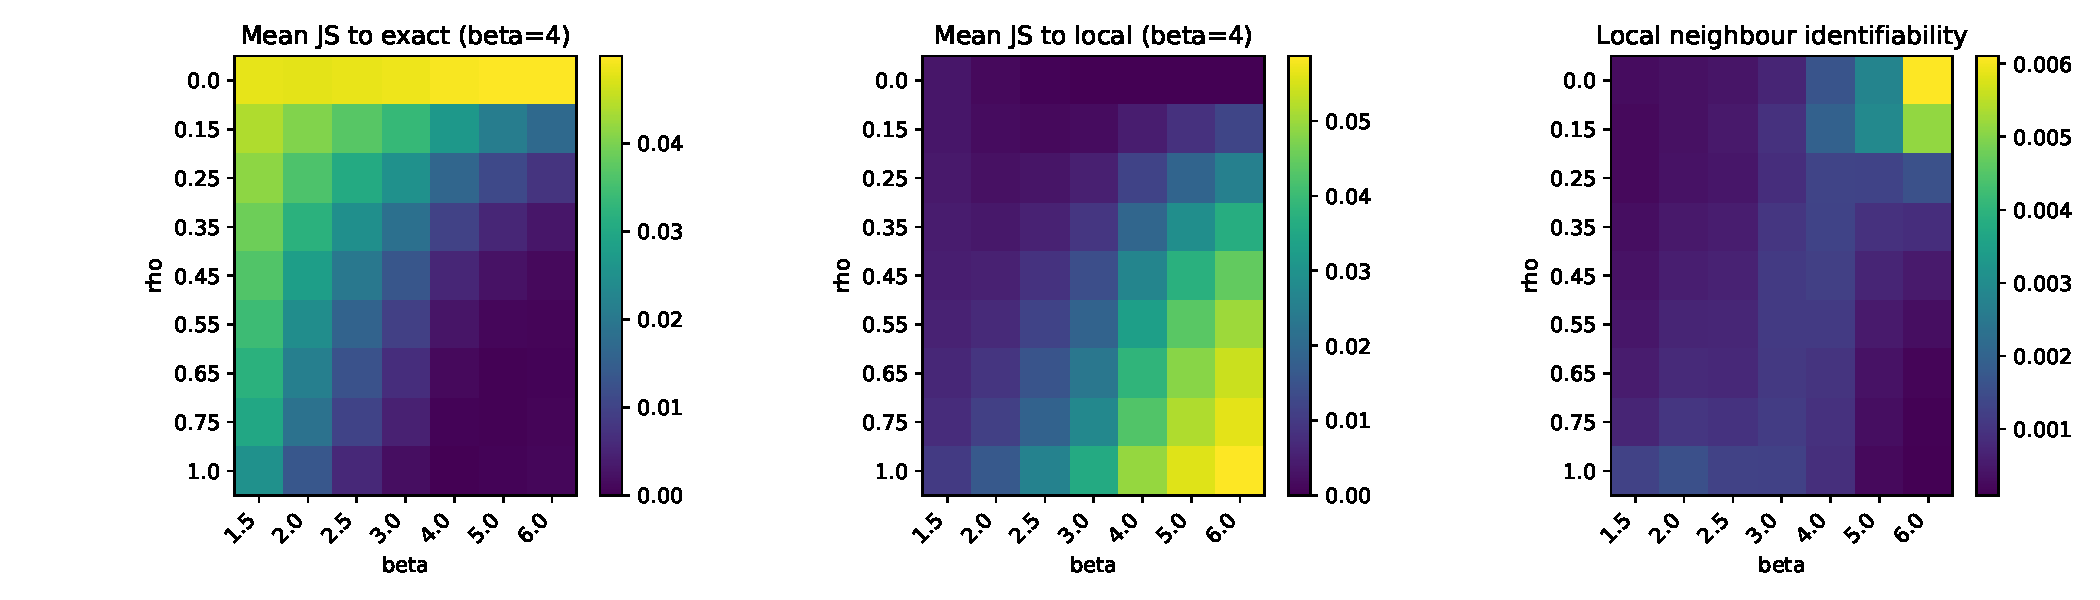
\includegraphics[width=\textwidth]{analysis-4-3_fig1_parameter_atlas.pdf}
\caption{Parameter atlas over the joint $\rho$--$\beta$ grid.}
\end{figure}

\begin{figure}[H]
\centering
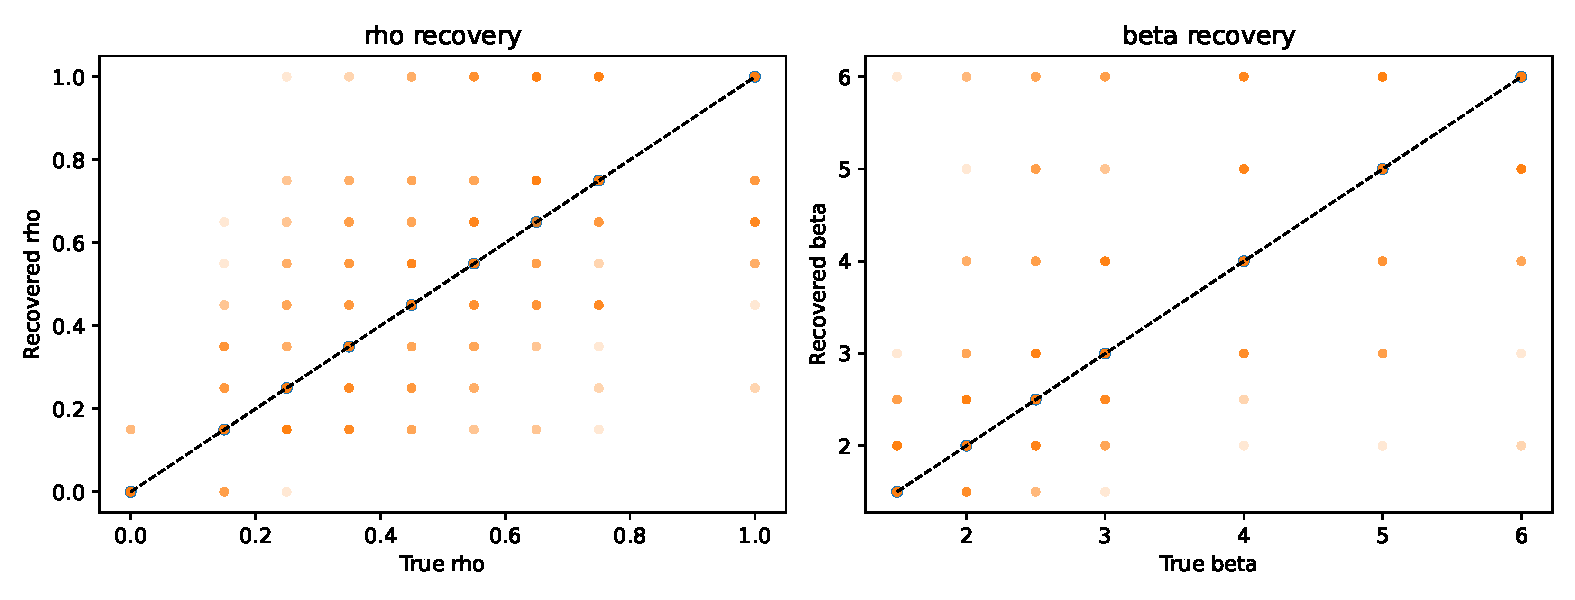
\includegraphics[width=0.88\textwidth]{analysis-4-3_fig2_recovery.pdf}
\caption{True-versus-recovered $\rho$ and $\beta$ values under noiseless and noisy synthetic data.}
\end{figure}

\section{Conclusions against the TODO}
\begin{enumerate}
    \item $\rho$ and $\beta$ are identifiable in principle on a targeted panel.
    \item The noisy regime shows a real tradeoff, especially for $\beta$.
    \item Family-level conclusions involving star rewrites survive $\beta$ optimisation better than subtle exact-versus-attenuation contrasts.
    \item Future fitting should either estimate $\rho$ and $\beta$ jointly or restrict analyses to the diagnostic panel identified here.
\end{enumerate}

\bibliographystyle{apalike}
\bibliography{../../manuscript/library}
\end{document}
